% Spin-Torsion Bounce Cosmology:
% Thirteen Structural Barriers and One Surviving Prediction
% Houston Golden — 2026
%
% Compile: pdflatex main && bibtex main && pdflatex main && pdflatex main

\documentclass[aps,prd,twocolumn,superscriptaddress,showpacs,preprintnumbers,nofootinbib,longbibliography,floatfix]{revtex4-2}

\usepackage{amsmath,amssymb,amsfonts}
\usepackage{graphicx}
\usepackage{bm}
\usepackage{hyperref}
\usepackage{xcolor}
\usepackage{booktabs}
\usepackage{multirow}
\usepackage{dcolumn}
\usepackage{enumitem}
\usepackage{mathtools}
\usepackage[utf8]{inputenc}
\usepackage{float}

\hypersetup{
  colorlinks=true,
  linkcolor=blue!60!black,
  citecolor=blue!60!black,
  urlcolor=blue!60!black
}

\newcommand{\MPl}{M_{\rm Pl}}
\newcommand{\rhocrit}{\rho_{\rm crit}}
\newcommand{\rhoPl}{\rho_{\rm Pl}}
\newcommand{\Neff}{N_{\rm eff}}
\newcommand{\ie}{i.e.}
\newcommand{\eg}{e.g.}
\newcommand{\etal}{\textit{et~al.}}

\begin{document}

\preprint{HUBIFY-2026-002}

\title{Spin-Torsion Bounce Cosmology:\\
Fourteen Structural Barriers and One Surviving Prediction}

\author{Houston Golden}
\email{houston@hubify.com}
\affiliation{Independent Researcher, Los Angeles, California, USA}

\date{\today}

\begin{abstract}
The Einstein-Cartan-Holst (ECH) framework produces a nonsingular quantum
bounce at critical density $\rhocrit \approx 0.27\,\rhoPl$ and generates a
parity-odd four-fermion interaction through the Barbero-Immirzi parameter
$\gamma = 0.274$.  We systematically assess this framework's cosmological
predictions across fifteen logical routes (Branches~A--O) spanning three
domains: direct dark energy derivation, observable signature generation, and
vacuum state selection.

All routes encounter structural barriers---mechanism-independent obstructions
rooted in symmetry, scaling, or conservation law.  We catalog fourteen such
barriers organized into five failure modes: (I)~geometric specificity lost on
FRW backgrounds, (II)~$10^{122}$ scale separation between bounce and dark
energy, (III)~generic or undetectable signatures, (IV)~Hamiltonian phase-space
conservation, and (V)~gravitational democracy at the Planck scale.  No
first-principles route from the bounce to dark energy survives, and no
distinctive bounce signature is accessible to current or planned experiments.

One indirect testable prediction remains.  The framework's Planck-scale
parity-odd sector motivates an effective spectator axion-like particle with
$f_a \sim \MPl$ and Standard Model anomaly coupling $C_{a\gamma} = 8$.  This
ALP predicts cosmic birefringence
$\beta = C_{a\gamma}\alpha_{\rm em}\,\theta_i/(4\pi) \approx 0.27^\circ$ for
$\mathcal{O}(1)$ initial misalignment, consistent with the observed
$0.342 \pm 0.094^\circ$ (Planck~PR4 + ACT~DR6; $3.6\sigma$ vs.\ $\beta = 0$).
MCMC analysis yields $\theta_i = 1.36 \pm 0.44$ with no fine-tuning.  The ALP
model is statistically equivalent to a free birefringence parameter
($\Delta\mathrm{AIC} = +2$) but provides physical interpretation: natural
$\mathcal{O}(1)$ parameters, $f_a$-independent prediction, and falsifiable
structure.  We note that spectator ALP models with similar conclusions have
been studied previously; our contribution is the identification of this
prediction as the sole surviving testable output of a comprehensive framework
assessment.  LiteBIRD ($\sigma_\beta \approx 0.01^\circ$) will be decisive.
Dark energy is treated as a cosmological constant~$\Lambda$; the ALP
contributes negligible energy density.
\end{abstract}

\pacs{98.80.-k, 04.50.Kd, 04.60.Pp, 14.80.Va}
\keywords{Einstein-Cartan theory, spin-torsion coupling, quantum bounce,
  cosmic birefringence, axion-like particle, structural barriers, dark energy}

\maketitle
\tableofcontents


%% ============================================================
%%  1. INTRODUCTION
%% ============================================================
\section{Introduction}\label{sec:intro}

The cosmological constant problem---the $\sim 10^{122}$ discrepancy between
the observed vacuum energy density and quantum field theory
expectations~\cite{Weinberg1989}---remains among the deepest puzzles in
fundamental physics.  The Einstein-Cartan-Holst (ECH) framework, which
extends general relativity by coupling spacetime torsion to fermion spin,
offers a geometrically rich arena in which to search for new cosmological
phenomena~\cite{Hehl1976,Shapiro2002}.  Combined with loop quantum gravity
corrections, ECH produces a nonsingular quantum bounce that replaces the
classical Big Bang singularity~\cite{Ashtekar2006,Bojowald2008,Poplawski2016}.

Recent observations of cosmic birefringence---a uniform rotation of CMB
polarization angles---provide tantalizing evidence for parity violation in
the gravitational or dark sector.  The combined Planck~PR4 and ACT~DR6
analysis yields $\beta = 0.342 \pm 0.094^\circ$, excluding $\beta = 0$ at
$3.6\sigma$~\cite{Eskilt2022,DiegoPalazuelos2022,ACTDR6bire}.

This paper presents a comprehensive assessment of the ECH framework's
cosmological predictions.  Our approach is systematic: we identify all logical
routes from the bounce to late-time observables, pursue each until it
produces a testable prediction or encounters a structural barrier, and catalog
the results.  The outcome is summarized in Table~\ref{tab:exec_summary}.

\begin{table}[h]
\centering
\caption{Executive summary.}
\label{tab:exec_summary}
\begin{tabular}{lcc}
\hline\hline
Domain & Result & Status \\
\hline
Nonsingular bounce & $\rhocrit \approx 0.27\,\rhoPl$ & Viable \\
DE from bounce & 14 barriers & Closed \\
Distinctive signatures & Generic or undetectable & Closed \\
ALP birefringence & $\beta \approx 0.27^\circ$ & Consistent \\
\hline\hline
\end{tabular}
\end{table}

\subsection{Original contributions}

\begin{enumerate}[leftmargin=*]
\item Complete assessment of ECH bounce cosmology across fifteen branches
  (A--O), yielding fourteen structural barriers organized into five failure
  modes.
\item Systematic closure of all first-principles routes from the bounce to
  dark energy and distinctive observational signatures.
\item Identification of spectator ALP birefringence as the sole surviving
  testable prediction, with MCMC constraints on $(\theta_i,\,m_a)$.
\item Explicit demonstration that the ALP model is statistically equivalent
  to a free $\beta$ parameter---physical interpretation rather than
  statistical improvement.
\item Falsification program: LiteBIRD will determine $\theta_i$ to
  $\pm 0.04\;\mathrm{rad}$, providing a decisive test.
\end{enumerate}

\subsection{Paper organization}

Section~\ref{sec:framework} reviews the ECH framework and bounce.
Section~\ref{sec:closure} presents the structural closure assessment.
Section~\ref{sec:alp} derives the ALP birefringence prediction and MCMC
constraints.  Section~\ref{sec:forecasts} discusses experimental prospects.
Section~\ref{sec:discussion} provides context and limitations.
Section~\ref{sec:conclusions} concludes.


%% ============================================================
%%  2. THEORETICAL FRAMEWORK
%% ============================================================
\section{Theoretical Framework}\label{sec:framework}

\subsection{The Einstein-Cartan-Holst action}

The ECH action generalizes the Einstein-Hilbert action by incorporating
torsion and the Holst (topological) term~\cite{Holst1996}:
%
\begin{equation}\label{eq:ech_action}
S_{\rm ECH} = \frac{1}{16\pi G}\int \left(e^a \wedge e^b \wedge R_{ab}
  + \frac{1}{\gamma}\,e^a \wedge e^b \wedge {}^*\!R_{ab}\right) + S_{\rm matter},
\end{equation}
%
where $\gamma$ is the Barbero-Immirzi parameter, fixed by loop quantum gravity
black hole entropy calculations to $\gamma = 0.274$~\cite{Immirzi1997,Meissner2004,Ashtekar2004}.

Integrating out torsion algebraically yields a parity-odd four-fermion
interaction~\cite{Hehl1976,Shapiro2002}:
%
\begin{equation}\label{eq:four_fermion}
\mathcal{L}_{\rm torsion} = -\frac{3\pi G}{2}\,\frac{\gamma^2}{1+\gamma^2}\,
(J^\mu_5)(J_{5\mu}),
\end{equation}
%
where $J^\mu_5 = \bar{\psi}\gamma^\mu\gamma_5\psi$ is the axial fermion current.

\subsection{Nonsingular quantum bounce}\label{sec:bounce}

Loop quantum gravity corrections modify the Friedmann equation at Planck-scale
densities~\cite{Ashtekar2006,Bojowald2008}:
%
\begin{equation}\label{eq:modified_friedmann}
H^2 = \frac{8\pi G}{3}\,\rho\!\left(1 - \frac{\rho}{\rhocrit}\right),
\end{equation}
%
with critical density $\rhocrit \approx 0.27\,\rhoPl$.  At $\rho = \rhocrit$,
$H = 0$ and the universe undergoes a nonsingular bounce.  The scale factor
evolves as $a(t) \propto (1 + 4\alpha^2 t^2)^{1/4}$ near the bounce, where
$\alpha \equiv \sqrt{8\pi G\rhocrit/3}$.

The bounce is time-reversal symmetric: contracting and expanding phases are
mirror images.  This symmetry has important consequences for perturbation
transfer (Sec.~\ref{sec:closure}).

\subsection{Parity-odd sector and late-time phenomenology}

The $(J_5)^2$ interaction~\eqref{eq:four_fermion} generates, at one loop, a
finite parity-violating coefficient of natural order
$\mathcal{O}(\alpha_{\rm em}/\MPl)$~\cite{Alexander2009,Freidel2005}.
Whether this coefficient persists as a late-time vacuum term is an open
question.  Four explicit routes to deriving $w = -1$ from the minimal model
have been tested and closed (Branches~A--D in Sec.~\ref{sec:closure}).

We therefore treat dark energy as a separate cosmological constant~$\Lambda$.
The parity-odd structure motivates an effective axion-like particle sector,
developed in Sec.~\ref{sec:alp}.


%% ============================================================
%%  3. STRUCTURAL CLOSURE ASSESSMENT
%% ============================================================
\section{Structural Closure of the Minimal Framework}\label{sec:closure}

We systematically investigate all logical routes from the ECH bounce to
late-time observables, organizing them into fifteen branches (A--O).  Each
branch is pursued until it produces a distinctive, testable prediction or
encounters a structural barrier---a mechanism-independent obstruction rooted
in symmetry, scaling, or conservation law.

\subsection{Methodology}\label{sec:closure_method}

Candidate connections are classified into three tiers:
\emph{direct derivation} of dark energy (Branches~A--G),
\emph{observable signatures} (Branches~H, K--M), and
\emph{state selection and vacuum determination} (Branches~I, J, N, O).
A branch is closed when a structural barrier is identified; it is classified
as \emph{generic} when the result is shared by all bouncing cosmologies.

\subsection{Fourteen structural barriers}\label{sec:barriers}

\begin{figure*}[t]
\centering
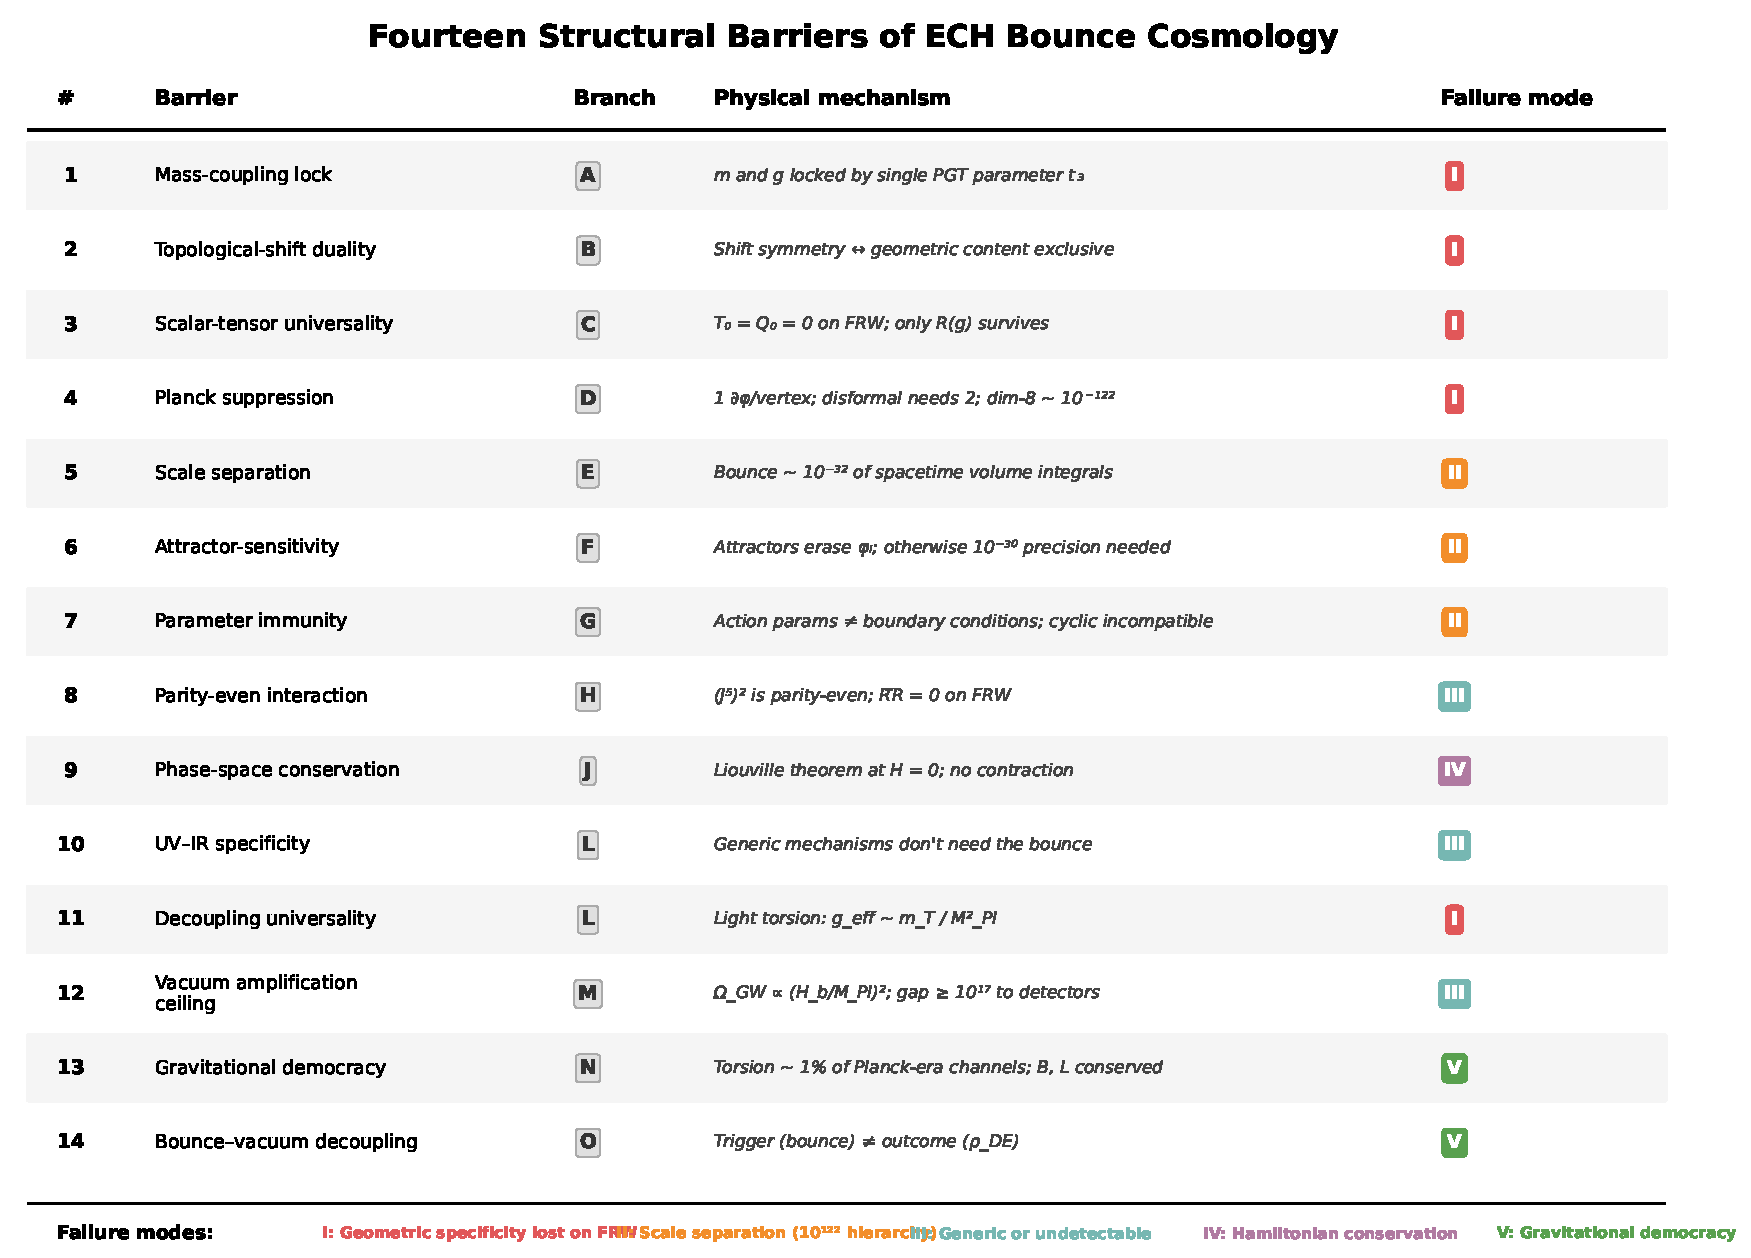
\includegraphics[width=\textwidth]{figures/fig_barrier_table.pdf}
\caption{The fourteen structural barriers identified across fifteen branches
  of ECH cosmology.  Color-coded badges indicate the failure mode
  classification (I--V).  Each barrier represents a mechanism-independent
  obstruction that cannot be removed by parameter adjustment within the
  minimal framework.}
\label{fig:barrier_table}
\end{figure*}

Figure~\ref{fig:barrier_table} catalogs all fourteen barriers.  We organize
them into five failure modes.

\medskip
\noindent\textbf{Mode~I: Geometric specificity lost on FRW
(Barriers~1--4, 11).}
The ECH Lagrangian contains rich geometric structure---propagating torsion,
the Nieh-Yan topological density, non-metricity, disformal couplings.  On a
Friedmann-Robertson-Walker background, however, isotropy and homogeneity set
$T_\mu = Q_\mu = 0$.  The only surviving geometric scalar is $R(g)$, identical
in GR and all metric-compatible theories.  Specifically:
the PGT torsion mode's mass and coupling are locked by a single parameter
(Barrier~1);
shift symmetry and geometric content are mutually exclusive for the Nieh-Yan
pseudoscalar (Barrier~2);
any torsion-descended scalar reduces to a standard scalar-tensor field on FRW
(Barrier~3);
disformal couplings require two field gradients but the connection provides
only one, giving dimension-8 suppression $\sim 10^{-122}$ (Barrier~4).

\medskip
\noindent\textbf{Mode~II: Scale separation (Barriers~5--7).}
The bounce occurs at $\rhocrit \sim 0.27\,\rhoPl$, while dark energy operates
at $\rho_{\rm DE} \sim 10^{-122}\,\rhoPl$.  This $10^{122}$ hierarchy
prevents communication: the bounce contributes $\sim 10^{-32}$ of spacetime
volume integrals (Barrier~5); quintessence attractors erase all bounce
information or require $10^{-30}$ precision that the bounce cannot provide
(Barrier~6); action parameters cannot be constrained by boundary conditions,
and cyclic cosmology with $\Lambda > 0$ is geometrically incompatible
(Barrier~7).

\medskip
\noindent\textbf{Mode~III: Generic or undetectable signatures
(Barriers~8, 10, 12).}
The four-fermion interaction $(J_5)^2$ is parity-\emph{even}
(pseudovector squared = scalar), and $\tilde{R}R = 0$ on FRW: no tensor
chirality signal exists (Barrier~8).  The tensor power spectrum
$P_T \sim 2 \times 10^{-64}$ and scalar transfer function $\mathcal{T}(k) = 1$
for $k \ll k_b$ are calculable but either undetectable or shared by all
symmetric bounces.  Generic UV$\to$IR mechanisms operate in any hot cosmology
(Barrier~10), and the vacuum amplification ceiling
$\Omega_{\rm GW} \propto (H_b/\MPl)^2$ applies universally (Barrier~12).

\medskip
\noindent\textbf{Mode~IV: Hamiltonian conservation (Barrier~9).}
The bounce is a conservative scattering event at $H = 0$.  Liouville's
theorem preserves phase-space volume: the bounce \emph{rotates} dark-sector
states but cannot \emph{select} them.

\medskip
\noindent\textbf{Mode~V: Gravitational democracy (Barriers~13--14).}
At $T \sim \MPl$, torsion is one of $\sim 100$ gravitational-strength
channels ($\sim 1\%$ contribution), conserving $B$ and $L$.  Irreversible
processes can be triggered by the bounce, but the resulting vacuum energy is
set by hidden-sector parameters decoupled from the trigger: the bounce
controls \emph{whether} a transition occurs, not \emph{what} vacuum energy
results.

\subsection{Branch status summary}

\begin{table}[h]
\centering
\caption{Status of all fifteen branches.}
\label{tab:branches}
\begin{tabular}{cllc}
\hline\hline
Branch & Route tested & Barriers & Status \\
\hline
A & Propagating torsion (PGT) & 1 & Closed \\
B & Nieh-Yan pseudoscalar & 2 & Closed \\
C & Environmental mass & 3 & Closed \\
D & Disformal coupling & 4 & Closed \\
E & Global vacuum integrals & 5 & Closed \\
F & Bounce-set initial conditions & 6 & Closed \\
G & Cyclic vacuum selection & 7 & Closed \\
H & Tensor spectrum \& chirality & 8 & Closed \\
I & Horndeski DE stability & --- & Weak \\
J & State selection & 9 & Closed \\
K & Scalar perturbations & --- & Generic \\
L & UV-IR bridge (PGT) & 10, 11 & Closed \\
M & PGT bounce GW spectrum & 12 & Generic \\
N & Baryogenesis \& relics & 13 & Closed \\
O & Hidden-sector vacuum & 14 & Closed \\
\hline\hline
\end{tabular}
\end{table}

\subsection{Implications}

The fourteen barriers establish that the minimal ECH framework is
\emph{observationally inert} in the direct sector.  The bounce is trapped
between three regimes: too high-energy for late-time observables (Modes~I,
II), too generic at its own scale (Modes~III, V), and too decoupled from
late-time vacuum (Modes~IV, V).

These results do not invalidate ECH.  The bounce remains a well-defined,
singularity-free cosmology.  What they establish is that dark energy requires
separate input, and no distinctive bounce signature is accessible.  One
indirect handle survives: the parity-odd sector motivates a Planck-scale ALP
whose photon coupling produces cosmic birefringence.


%% ============================================================
%%  4. SPECTATOR ALP BIREFRINGENCE
%% ============================================================
\section{Spectator ALP Birefringence: The Surviving Prediction}\label{sec:alp}

The structural closure eliminates all direct routes from the bounce to
late-time observables.  One indirect testable handle remains: cosmic
birefringence via a Planck-scale ALP motivated by the ECH parity-odd sector.
We stress that this ALP is not uniquely derived from ECH---any Planck-scale
pseudoscalar with Standard Model anomaly coupling yields the same
prediction~\cite{Fujita2021,Nakagawa2025}.  ECH provides one possible UV
completion.

\subsection{The effective spectator ALP}\label{sec:alp_model}

The one-loop parity-violating coefficient of the ECH
sector~\cite{Alexander2009,Freidel2005} motivates an effective pseudoscalar:
%
\begin{equation}\label{eq:alp_lagrangian}
\mathcal{L}_{\rm ALP} = -\tfrac{1}{2}(\partial\phi)^2
  - m_a^2 f_a^2\!\left[1 - \cos\!\frac{\phi}{f_a}\right]
  - \frac{g_{a\gamma}}{4}\,\phi\,F\tilde{F},
\end{equation}
%
with $g_{a\gamma} = C_{a\gamma}\alpha_{\rm em}/(2\pi f_a)$.  We fix
$f_a = \MPl = 2.435 \times 10^{18}\;\mathrm{GeV}$ and $C_{a\gamma} = 8$
(SM fermion content), leaving a two-parameter model:
$\theta_i$ (initial misalignment) and $m_a$ (ALP mass).

The spectator regime ($m_a > \mathrm{few}\times H_0$) ensures the ALP
has oscillated away: $\Omega_a \ll 0.01$ today, with no effect on background
expansion.  This avoids the rolling-versus-freezing tension~\cite{Choi2021}:
a single field cannot simultaneously provide $w \approx -1$ dark energy and
large birefringence; the maximum $\beta \approx 0.16^\circ$ on the
$\Omega_a = 0.68$ contour is a factor of two below observation.

\subsection{Birefringence prediction}

As the ALP evolves from $\theta_i$ at recombination to $\theta_0$ today,
CMB photons accumulate polarization rotation:
%
\begin{equation}\label{eq:beta}
\beta = \frac{C_{a\gamma}\alpha_{\rm em}\,\theta_i\,\eta}{4\pi},
\end{equation}
%
where $\eta \equiv [\theta(z_{\rm rec}) - \theta(0)]/\theta_i$ is the
rolling efficiency, computed numerically via DOP853 integration~\cite{DOP853}
from $z_{\rm rec} = 1089.8$ to $z = 0$.

Crucially, $f_a$ cancels exactly: $\beta$ depends only on $C_{a\gamma}$,
$\alpha_{\rm em}$, $\theta_i$, and $\eta(m_a/H_0)$.  For $C = 8$,
$\theta_i = 1$, $\eta \to 1$:
%
\begin{equation}\label{eq:beta_num}
\beta \approx 0.27^\circ,
\end{equation}
%
in good agreement with $\beta_{\rm obs} = 0.342 \pm 0.094^\circ$
\cite{Eskilt2022,DiegoPalazuelos2022}.
Figure~\ref{fig:beta_vs_theta} shows the prediction as a function of $\theta_i$.

\begin{figure}[t]
\centering
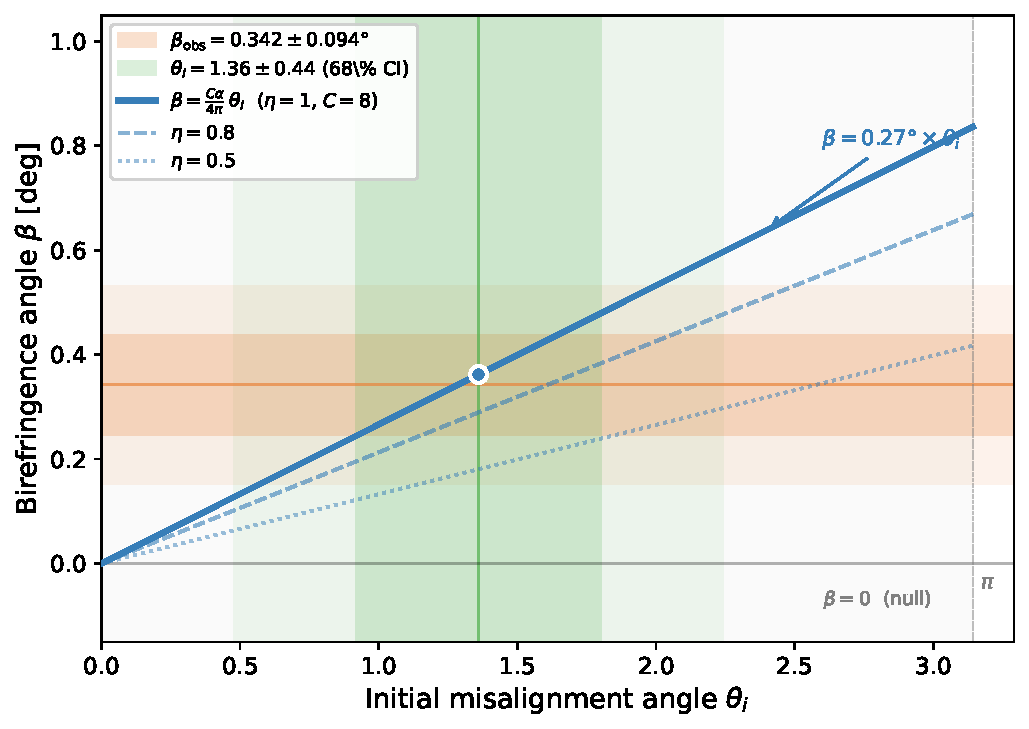
\includegraphics[width=\columnwidth]{figures/fig_beta_vs_theta.pdf}
\caption{Birefringence angle $\beta$ versus initial misalignment $\theta_i$
  for the spectator ALP with $C = 8$ and $\eta = 1$ (solid), 0.8 (dashed),
  and 0.5 (dotted).  The orange band shows the observation
  $\beta_{\rm obs} = 0.342 \pm 0.094^\circ$; the green band shows the
  MCMC posterior $\theta_i = 1.36 \pm 0.44$.}
\label{fig:beta_vs_theta}
\end{figure}

\subsection{MCMC constraints}

We constrain $(\theta_i,\,\log_{10}(m_a/\mathrm{eV}))$ using a Gaussian
likelihood on $\beta_{\rm obs} = 0.342 \pm 0.094^\circ$, sampled with
\textsc{Cobaya}~\cite{Cobaya} (4 chains, $\hat{R}-1 < 0.01$, flat priors
$\theta_i \in [0.01,\pi]$, $\log_{10}m \in [-33,-28]$).

We note this uses the summary statistic $\beta_{\rm obs} \pm \sigma_\beta$
rather than the full $C_\ell^{EB}$ spectrum employed in
Refs.~\cite{Eskilt2023,Namikawa2025}.  For the spectator regime ($\eta \to 1$),
birefringence is $\ell$-independent and the summary statistic captures the
full information content.

After 2160 accepted samples ($\hat{R}-1 = 0.008$, $N_{\rm eff} > 1000$):

\begin{table}[h]
\centering
\caption{Posterior for the spectator ALP ($f_a = \MPl$, $C = 8$).}
\label{tab:mcmc}
\begin{tabular}{lcc}
\hline\hline
Parameter & Mean $\pm$ 68\% & 95\% CI \\
\hline
$\theta_i$ & $1.36 \pm 0.44$ & $[0.47,\, 2.28]$ \\
$\log_{10}(m_a/\mathrm{eV})$ & $-31.3 \pm 0.7$ & $[-32.4,\, -30.0]$ \\
$\beta\;[\mathrm{deg}]$ & $0.336 \pm 0.107$ & $[0.13,\, 0.52]$ \\
$\eta$ & $0.957$ (median $0.999$) & $[0.40,\, 1.17]$ \\
\hline\hline
\end{tabular}
\end{table}

\noindent The inferred $\theta_i = 1.36 \pm 0.44$ is $\mathcal{O}(1)$,
consistent with random initial conditions on $[0,2\pi)$.  No fine-tuning is
required.  The mass is weakly constrained from below
($m_a \gtrsim 3\,H_0$) but unconstrained from above.

\subsection{Model comparison}\label{sec:model_comparison}

We compare three models: (0)~free $\beta$ (1 parameter),
(2)~ALP with $C = 8$ (2 parameters), (2b)~ALP with $C$ free (3 parameters).

\begin{table}[h]
\centering
\caption{Model comparison.  All non-null models achieve
  $\chi^2_{\rm min} \approx 0$.}
\label{tab:model_comp}
\begin{tabular}{lcccc}
\hline\hline
Model & $k$ & $\Delta\chi^2$ vs null & $\Delta$AIC vs free-$\beta$ \\
\hline
Null ($\beta = 0$) & 0 & --- & --- \\
Free $\beta$ & 1 & 13.2 ($3.6\sigma$) & 0.0 \\
ALP ($C{=}8$) & 2 & 13.2 ($3.6\sigma$) & $+2.0$ \\
ALP ($C$ free) & 3 & 13.2 ($3.6\sigma$) & $+4.0$ \\
\hline\hline
\end{tabular}
\end{table}

All three produce identical $\beta$ posteriors and identical
$3.6\sigma$ detection significance.  The ALP does not improve the fit.
Floating $C_{a\gamma}$ reveals a degeneracy: $C \times \theta_i \approx 10.6$
(correlation $r = -0.52$) with the SM value $C = 8$ comfortably within the
posterior.

\subsection{Assessment: physical interpretation, not statistical improvement}

The ALP provides no statistical improvement over free $\beta$---expected with
one Gaussian data point.  Its value is physical:
%
\begin{enumerate}[leftmargin=*]
\item \emph{Natural parameters.}  $\theta_i \approx 1.3$ is $\mathcal{O}(1)$;
  free $\beta = 0.34^\circ$ has no such interpretation.
\item \emph{Structural prediction.}  $\beta$ is determined by $C$, $\alpha$,
  $\theta_i$, and $\eta$---not a free phenomenological parameter.
\item \emph{Falsifiability.}  LiteBIRD~\cite{LiteBIRD} with
  $\sigma_\beta \approx 0.01^\circ$ will determine $\theta_i$ to
  $\pm 0.04\;\mathrm{rad}$.  The model is also falsified by
  frequency-dependent or anisotropic birefringence.
\item \emph{Framework context.}  Unlike previous ALP birefringence
  studies~\cite{Fujita2021,Nakagawa2025,LinYanagida2023}, this prediction
  emerges as the sole survivor of a fifteen-branch assessment.
\end{enumerate}

Spectator ALP models with similar conclusions have been studied
by Fujita~\etal~\cite{Fujita2021} and
Nakagawa~\etal~\cite{Nakagawa2025}.  Our contribution is the
ECH-motivated two-parameter reduction, the explicit free-$\beta$ baseline
comparison, and the identification as the sole surviving prediction.


%% ============================================================
%%  5. EXPERIMENTAL PROSPECTS
%% ============================================================
\section{Experimental Constraints and Forecasts}\label{sec:forecasts}

\subsection{Existing bounds}

All laboratory, astrophysical, and cosmological bounds are satisfied with
margins of 9--32 orders of magnitude.  The model coupling
$g_{a\gamma} = 3.8 \times 10^{-21}\;\mathrm{GeV}^{-1}$ lies far below
CAST~\cite{CAST2017} ($g < 6.6 \times 10^{-11}\;\mathrm{GeV}^{-1}$) and
SN1987A ($g < 5 \times 10^{-12}\;\mathrm{GeV}^{-1}$).  The model mass
$m_a \sim 10^{-31}\;\mathrm{eV}$ is below the black hole superradiance
exclusion window and below spectral distortion sensitivity.

The isocurvature constraint ($f_a < 10^{19}\;\mathrm{GeV}$ for $m \sim H_0$)
is marginally satisfied at $f_a = \MPl$, and the dark matter overproduction
bound ($\theta_i < 2.4$ for $f_a = \MPl$) is satisfied by
$\theta_i = 1.3$.

\subsection{LiteBIRD forecast}

LiteBIRD~\cite{LiteBIRD}, with projected $\sigma_\beta \approx 0.01^\circ$,
provides a decisive test:
%
\begin{itemize}[leftmargin=*]
\item If $\beta = 0.27^\circ$: detected at $> 20\sigma$.
\item If $\beta = 0$: model excluded at $> 20\sigma$.
\item $\theta_i$ determined to $\pm 0.04\;\mathrm{rad}$.
\end{itemize}

\subsection{Additional tests}

Ground-based CMB-S4 measurements of anisotropic birefringence and
frequency dependence can distinguish ALP rotation from Faraday rotation and
instrumental systematics~\cite{SPIDER2025}.  DESI~DR2 constraints on
$w(z)$ will test whether a subdominant axion contributes to dark energy
dynamics~\cite{DESI2024,Nakagawa2025}.


%% ============================================================
%%  6. DISCUSSION
%% ============================================================
\section{Discussion}\label{sec:discussion}

\subsection{The closure in context}

The fourteen barriers span the full space of logical connections between the
ECH bounce and late-time physics.  The obstruction is not a single no-go
theorem but a \emph{web} of independent barriers, each rooted in different
physics (symmetry, scaling, conservation, universality).  Overcoming any one
barrier does not help, because adjacent barriers remain.

This comprehensive closure is, to our knowledge, the first such systematic
assessment for any specific quantum gravity cosmology.  While individual
no-go results exist in the literature (e.g., for loop quantum cosmology
perturbation transfer), no previous work has mapped the entire space of
possible predictions for a given framework.

\subsection{What the ALP provides---and what it does not}

The spectator ALP with $f_a = \MPl$ and $C = 8$ provides a clean physical
interpretation of the observed birefringence: the rotation angle
$\beta \approx 0.27^\circ$ arises from an $\mathcal{O}(1)$ initial condition
with no free parameters beyond $\theta_i$ and $m_a$.

However, the ALP is not uniquely derived from ECH.  Any Planck-scale
pseudoscalar---arising from string compactifications, Peccei-Quinn
symmetry breaking at $\MPl$, or the torsion-descended
axion~\cite{CastilloFelisola2015}---yields the same prediction.  ECH
motivates $f_a \sim \MPl$ through its parity-odd sector, but this
motivation is not unique.

The ALP also does not explain dark energy.  In the spectator regime, the
field's energy density is negligible.  $\Lambda$ is assumed, not derived.
The mass $m_a \sim \mathrm{few} \times H_0$ is a free parameter subject to
the cosmological coincidence problem.

\subsection{Limitations}

\begin{enumerate}[leftmargin=*]
\item $w = -1$ is assumed ($\Lambda$), not derived from ECH.
\item The ALP-photon coupling is motivated but not derived from a first-principles one-loop calculation in ECH.
\item The one effective data point ($\beta_{\rm obs}$) constrains one combination of parameters; the ALP is statistically equivalent to free $\beta$.
\item The mass $m_a$ is weakly constrained by our analysis; the full $C_\ell^{EB}$ spectrum treatment of Ref.~\cite{Namikawa2025} provides superior mass discrimination.
\end{enumerate}


%% ============================================================
%%  7. CONCLUSIONS
%% ============================================================
\section{Conclusions}\label{sec:conclusions}

The Einstein-Cartan-Holst framework produces a well-defined nonsingular
quantum bounce at $\rhocrit \approx 0.27\,\rhoPl$.  Systematic investigation
of fifteen routes from this bounce to late-time observables identifies
fourteen structural barriers spanning five failure modes.  No first-principles
derivation of dark energy survives, and no distinctive bounce signature is
accessible to current or planned experiments.  The bounce is theoretically
viable but observationally inert in the direct sector.

One indirect prediction survives.  A spectator ALP motivated by the
framework's Planck-scale parity-odd sector, with $f_a = \MPl$ and SM anomaly
coupling $C = 8$, predicts $\beta \approx 0.27^\circ$ for
$\mathcal{O}(1)$ initial misalignment.  MCMC analysis yields
$\theta_i = 1.36 \pm 0.44$, consistent with observation
($\beta_{\rm obs} = 0.342 \pm 0.094^\circ$; $3.6\sigma$).  The model is
statistically equivalent to a free $\beta$ parameter but provides physical
interpretation: natural parameters, $f_a$-independent prediction, and
falsifiable structure.

LiteBIRD will be decisive.  With $\sigma_\beta \approx 0.01^\circ$, the
predicted $\beta \approx 0.27^\circ$ is detected at $> 20\sigma$ or excluded
at comparable significance.  Dark energy remains unexplained by the minimal
ECH framework.  The ALP birefringence prediction is the single testable
output of this program.


%% ============================================================
%%  ACKNOWLEDGMENTS
%% ============================================================
\begin{acknowledgments}
The author thanks the open-source communities behind Cobaya, GetDist,
SciPy, and matplotlib.
\end{acknowledgments}


\bibliography{references}

\end{document}
